\documentclass[12pt,a4paper,twoside,openright]{report}

%%%%%%% Import packages %%%%%%%
\usepackage{graphicx}
\usepackage{epsfig}
\usepackage{epstopdf,amsfonts,array,multirow,amsmath,tabularx,setspace,amssymb,enumerate,csquotes}
	
% \usepackage{url}
% \usepackage{bbm}
% \usepackage{eufrak}
% \usepackage{marvosym}
% \usepackage{moderncvcompatibility}

%% packages with settings
% Inline listing package
% \usepackage[inline]{enumitem}
\usepackage{listings}
% Page geometry
\usepackage{geometry}
\setlength{\evensidemargin}{0.0cm}
\setlength{\oddsidemargin}{0.0cm}
\setlength{\topmargin}{-1.27cm}
\setlength{\headheight}{32pt}
\setlength{\headsep}{1em} %% Setting for gap in header and main body%%
\setlength{\textheight}{24.0cm}
%\setlength{\textwidth}{14.65cm}
\setlength{\footskip}{1.5cm}
\setlength{\parindent}{1.5em}
\setlength{\parskip}{1em}

% Set line spacing to 1.25 because
% with 12pt font, 1.5 spacing is too large
\setstretch{1.25}

\usepackage{fancyhdr}
\usepackage[usenames,dvipsnames]{xcolor}
\usepackage{relsize}
\usepackage{bigints}

% Packages for table of contents
\setcounter{tocdepth}{3}

\usepackage[nottoc]{tocbibind}
\usepackage[titles,subfigure]{tocloft}

\makeatletter
\newlength{\@chapterlength} % Original Magic Value - RMR
\setlength{\@chapterlength}{1.5em} % This code adds space for \@chapapp for toc entries
\newcommand\@chapterheadsmark{1}
\ifnum \@chapterheadsmark = 1
\settowidth{\@chapterlength}{\@chapapp}
\addtolength{\@chapterlength}{3.8em} % Space between toc labels and values
\fi
% \def\l@chapter{\pagebreak[3]\vskip 1em plus 1pt \@dottedtocline{0}{0em}{1.5em}}
% \def\l@chapter{\pagebreak[3]\vskip 1em plus 1pt \@dottedtocline{0}{0em}{\@chapterlength}}

\def\l@section{\@dottedtocline{1}{\@chapterlength}{2.3em}}

\newlength{\@subsectionlength}
\setlength{\@subsectionlength}{\@chapterlength}
\addtolength{\@subsectionlength}{2.3em}
\def\l@subsection{\@dottedtocline{2}{\@subsectionlength}{3.2em}}

\newlength{\@subsubsectionlength}
\setlength{\@subsubsectionlength}{\@chapterlength}
\addtolength{\@subsubsectionlength}{5.5em}
\def\l@subsubsection{\@dottedtocline{3}{\@subsubsectionlength}{4.1em}}

\newlength{\@paragraphlength}
\setlength{\@paragraphlength}{\@chapterlength}
\addtolength{\@paragraphlength}{8.5em}
\def\l@paragraph{\@dottedtocline{4}{\@paragraphlength}{5em}}

\newlength{\@subparagraphlength}
\setlength{\@subparagraphlength}{\@chapterlength}
\addtolength{\@subparagraphlength}{10.5em}
\def\l@subparagraph{\@dottedtocline{5}{\@subparagraph}{6em}}
\makeatother

\renewcommand\cftchappresnum{\chaptername~}
\newlength\mylength
\settowidth\mylength{\cftchappresnum\cftchapaftersnum\qquad}
\addtolength\cftchapnumwidth{\mylength}

\usepackage[acronym,nomain,toc]{glossaries}
\makeglossaries
\usepackage[intoc]{nomencl}
\makenomenclature
\renewcommand{\nomname}{List of Symbols}
\usepackage[toc,page]{appendix}

% Packages for floats like figures and tables
\usepackage{float}
\usepackage{caption}
% \usepackage[center]{caption}
% \usepackage{longtable}
% \usepackage{subfig}
\usepackage{subfigure}
% \usepackage{subcaption}
% \usepackage[chapter]{algorithm}
\usepackage{algpseudocode}
% \usepackage{algorithmic}

\usepackage[base]{babel}
\usepackage{lipsum,blindtext} % just to generate text for the example

\usepackage{color}   %May be necessary if you want to color links

\usepackage{datetime}
\newdateformat{thisdate}{%
	\twodigit{\THEDAY}}
\newdateformat{thismonthdigit}{%
	\twodigit{\THEMONTH}}
\newdateformat{thismonth}{%
	\monthname[\THEMONTH]}
\newdateformat{thisyear}{%
	\THEYEAR}

% \usepackage{cite}
% \usepackage{notoccite}
\usepackage[backend=biber, style=ieee, sorting=none, defernumbers=true]{biblatex}
\addbibresource{bibliography.bib}

% Hyperref should be the last package to be loaded
\usepackage{hyperref}
% \hypersetup{
% 	breaklinks=true,
%     colorlinks=true, %set true if you want colored links
%     linktoc=all,     %set to all if you want both sections and subsections linked
%     linkcolor=black,  %choose some color if you want links to stand out
%     citecolor=black,
%     urlcolor=black
% }

\hypersetup{linktoc=all, colorlinks=true, linkcolor=Black, citecolor=teal, urlcolor=red}


\DeclareMathOperator{\arccot}{arccot}
\DeclareMathOperator{\sinc}{sinc}
\DeclareMathOperator*{\argmin}{arg\;min}
\DeclareMathOperator*{\argmax}{arg\;max}

\newtheorem{theorem}{Theorem}[chapter]
\newtheorem{proposition}{Proposition}[chapter]
\newtheorem{lemma}{Lemma}[chapter]
\newtheorem{definition}{Definition}[chapter]
\newtheorem{prop}{Proposition}
%-------------------------------------------------------------------

%\flushbottom
%--------------------------------------------------------------------------
\raggedbottom                               % (Remove Unnecessary space b/w paragraphs)
%--------------------------------------------------------------------------
\begin{document}

% --------- Title and abstract etc in the front matter ----------- %
\pagenumbering{gobble}
% TITLE PAGE
\begin{titlepage}
\begin{center}

{\fontencoding{T1}\fontfamily{pzc}\fontseries{m}\fontshape{n}\selectfont
\huge \bfseries Tooth Decay Detection Using Different YOLO Algorithms}\\
\vspace*{1cm}

{\large  \itshape CSE498R report submitted in partial fulfillment of the requirements for the degree}\\
\vspace*{0.5cm}
{\large \itshape {of}}\\
\vspace*{0.5cm}

{\fontencoding{T1}\fontfamily{pzc}\fontseries{m}\fontshape{n}\selectfont
\huge \bfseries Bachelor of Science in Computer Science and Engineering}\\
\vspace*{0.5cm}

{\large \itshape {by}}\\
\vspace*{0.5cm}
\begin{center}

{\large \bfseries Md Sazid Ahmed Tonmoy }\\
{\large \bfseries ID: 1911498042}\\
\par\end{center}
\vspace*{0.5cm}

{\large Under the guidance of\\}
\vspace*{0.2cm}

{\Large \bfseries Dr. Sifat Momen\\}
{\Large \bfseries Associate Professor\\}

\vspace*{1.0cm}


\includegraphics[scale=0.6]{nsu.png}
\vspace*{0.5cm}

\textsc{ \bfseries{DEPARTMENT OF ELECTRICAL & COMPUTER ENGINEERING\\
NORTH SOUTH UNIVERSITY\\Bashundhara, Dhaka-1229, Bangladesh\\}}
{ \bfseries Summer {\thisyear\today}\\}
\vspace*{0.1cm}

\end{center}
\end{titlepage}




%%%%%%%%%%%% Front Matter %%%%%%%%%%%%
\pagenumbering{roman}
% Page 5 : Approval of the DAC

% \chapter*{} is needed to link the hyperlinks in contents to the corresponding pages properly.
\chapter*{}
\vspace*{-5cm}
% \thispagestyle{empty}

{\centering 
\includegraphics[width=\linewidth, scale=1]{01_Declaration/letterhead.png}}
{\hrule width \hsize height 1.5pt \kern .5mm \hrule width \hsize height 1.5pt}
\vspace*{2ex}
\begin{center}
\textbf{\Large DECLARATION}
\end{center}
\vspace{2ex}
It is hereby acknowledged that: 
\begin{enumerate}[a.]
	\item No illegitimate procedure has been practiced during the preparation of this document.
	\item This document does not contain any previously published material without proper citation.
	\item This document represents our own accomplishment while being Undergraduate Students in the North South University.
\end{enumerate}
Sincerely,\\
\vspace{10em}
\begin{minipage}[t]{0.35\textwidth}
\end{minipage}%
\hfill
\begin{minipage}[t]{0.55\textwidth}
    \raggedleft
    \hrule\vspace{2ex}
     \textbf{Md Sazid Ahmed Tonmoy} \\
     \textbf{ID: 1911498042}
\end{minipage}
\addcontentsline{toc}{chapter}{Declaration}
\let\cleardoublepage\clearpage


% Page 7: Certificate on department letterhead

\chapter*{}
\vspace*{-5cm}
% \thispagestyle{empty}
% {~} % Buffer blank character to prevent horizontal underflow due to next \vspace
% \vspace{10em} % Increase if the dept. letterhead requires more space


{\centering 
\includegraphics[width=\linewidth, scale=1]{02_Approval/letterhead.png}}
{\hrule width \hsize height 1.5pt \kern .5mm \hrule width \hsize height 1.5pt}

\vspace*{2ex}
\begin{center}
\textbf{\Large Approval}
\end{center}

\par This is to certify that the CSE498R report entitled Tooth Decay Detection Using Different YOLO Algorithms, submitted by Md Sazid Ahmed Tonmoy (ID: 1911498042) is undergraduate students of the Department of Electrical & Computer Engineering, North South University. This report partially fulfil the requirements for the degree of Bachelor of Science in Computer Science and Engineering on September 11, 2022, and has been accepted as satisfactory.

\vspace{4em}
\begin{minipage}[t]{0.35\textwidth}
    Date: \\
\end{minipage}%
\hfill
\begin{minipage}[t]{0.55\textwidth}
    \raggedleft
    \hrule\vspace{2ex}
     \textbf{Dr. Sifat Momen} \\
    Associate Professor \\
 	Department of Electrical & Computer Engineering \\
 	North South University \\
 	Dhaka, Bangladesh
	

     \vspace{5em}
     \hrule\vspace{2ex}
     \textbf{Dr. Rajesh Palit} \\
    Professor and Chair \\
 	Department of Electrical & Computer Engineering \\
 	North South University \\
 	Dhaka, Bangladesh
\end{minipage}

\addcontentsline{toc}{chapter}{Certificate}

\let\cleardoublepage\clearpage

 
%%%%%%%%%%%% Abstract %%%%%%%%%%%%
\setstretch{2}  % double spacing
\chapter*{\centering Abstract}

\pagestyle{fancy}
\fancyhf{}
\fancyhead[LO,RE]{Abstract}
\fancyhead[LE,RO]{\thepage}

\addcontentsline{toc}{chapter}{Abstract}

Early detection and identification of eye disorders using fundus pictures is among ophthalmologists’ most difficult responsibilities. However, eye illness diagnosis by hand is challenging, time-consuming, and error-prone. For the purpose of employing fundus pictures for early identification of different ocular disorders, a computer-aided automated ocular disease detection system is necessary. Such a system can now be accomplished because to deep learning algorithms’ improved picture categorization skills. Four deep learning-based models for pinpointing ocular diseases are presented in this work. For this work, we used the ODIR dataset, which consists of 5000 fundus images. we took 3404 fundus images divided into 5 distinct groups, to train cutting-edge image classification algorithms including Resnet-50, MobileNetV2, and VGG-19.\\
\textbf{Index Terms: }Ocular Disease Classification, Color Fundus
Photography, Ocular Disease Detection, Convolutional Neural
Networks, VGG-19, Resnet-50, MobileNetV2, Deep Transfer
Learning



%%%%%% Table of Contents %%%%%%
%%%%%%% To create 1.5 spacing in contents
\setstretch{1.5}

%%%%%%%%%% To rename Table of Contents
\renewcommand{\contentsname}{Table of Contents}
% \renewcommand{\contentsname}{Contents}
%%%%%%%%%%
\tableofcontents
\addcontentsline{toc}{chapter}{\contentsname}
\pagestyle{fancy}
\fancyhf{}
\fancyhead[LO,RE]{\contentsname}
\fancyhead[LE,RO]{\thepage}

\listoftables
\listoffigures
\pagestyle{fancy}
\fancyhf{}
\fancyhead[LO,RE]{List of Tables}
\fancyhead[LE,RO]{\thepage}



% %%%%%% List of Algorithms %%%%%%
% \chapter*{}
% \addcontentsline{toc}{chapter}{List of Algorithms}
% \listofalgorithms
% \newpage



\let\cleardoublepage\clearpage


\pagenumbering{arabic}
%%%%%%%% To create double spacing in chapters
\setstretch{2}

% Fancy header
\pagestyle{fancy}
\renewcommand{\sectionmark}[1]{\markright{\thesection~#1}{}}
\renewcommand{\chaptermark}[1]{\markboth{\chaptername~\thechapter~-~#1}{}}
\fancyhf{}
%\fancyhead[RE]{\leftmark}
%\fancyhead[LO]{\rightmark}
\fancyhead[LE,RO]{\thepage}

%%%%%% Chapters %%%%%%
%% Remove any command starting with "\lipsum"
%% from the chapter text. They are used to generate
%% junk test paragraphs


\chapter{Introduction}


Various ocular diseases are capable of causing permanent and irreversible damage to the patient’s vision, and in extreme cases, they can even lead to blindness [1-3]. Although effective treatments are available for these ocular diseases, these treatment options can only be implemented if the disease is diagnosed as early as possible. Ocular diseases are primarily diagnosed using color fundus photography or CFP [4]. This technique is utilized in order to record the interior surface of the human eye so that various types of possible ocular diseases can be detected [5]. Although this method of diagnosis is effective, it’s still quite difficult to detect certain ocular diseases using CFP. Some of the most prevalent ocular diseases, such as cataracts, myopia, and diabetic retinopathy, are difficult to diagnose as they show very few initial symptoms. [6] Moreover, the process of manually inspecting and detecting ocular diseases is a laborious task, and this process is not that accurate [7].\\ In recent times, deep learning-based neural network models have shown promising results in medical image classification and object detection. Moreover, that is why convolutional neural network-based models have been extensively studied for ocular disease detection. Given this, it’s critical to offer these people affordable or free complete eye care treatments. Deep-learning-based algorithms are becoming more common in medical image analysis. Deep-learning-based models have been demonstrated to perform well in numerous tasks such object recognition, sentiment analysis [8], medical picture classification [9], and illness diagnosis [10]. One of the most important steps in minimizing an ophthalmologist’s workload is the automated diagnosis of diseases. Without the need for human interaction, illnesses may be detected using deep learning and computer vision technology. Only a small number of these studies have been able to fully diagnose [11] more than one eye illness, despite the fact that many of them have produced encouraging results. To accurately detect diverse eye conditions, more study is required to examine the many elements of fundus imaging [12]. This study suggests a system that uses deep learning to recognize different eye diseases. Multilabel categorization has been used as a different strategy [13]. The ocular disease’s datasets [14–15] are quite unbalanced. This imbalance makes it difficult to accurately identify or classify sickness or even a normal picture. This method is not recommended for broad classification problems due to its low accuracy.\\
As a result, our study initially balanced the dataset by training the classes on the pretrained Resnet50, VGG-19, and MobilenetV2 architecture with the same amount of data for each class. By selecting the equal number of photos for each classes, we first loaded the dataset and the associated image into the dataset. For the VGG-19, Resnet50, and Mobilenetv2 models in this work, the transfer learning approach was used. The accuracy of each class rose once we correctly balanced the dataset. The remaining portions of the essay are structured as follows: The relevant work for this study is displayed in Section 2. Dataset’s description is displayed in Section3. All the tools and techniques are extensively covered in Section 4. After discussing our study’s results and performance analysis in Section 5. Section 6 brings our work's deployment and Section 7 brings our work to a close.



\newpage
%\newpage\null\newpage

\chapter{LITERATURE REVIEWS}
% \graphicspath{{Chapter_2/Vector/}{Chapter_2/}}

An overview, a summary, and an assessment of the state of knowledge in a particular field of study make up a literature review. It could also highlight methodological concerns and make recommendations for further study.In this chapter, we have reviewed some papers related to our work.


\section{Deep Learning-Based Dental Plaque Detection on Primary Teeth: A Comparison With Clinical Assessments} Wenzhe You and his team aimed to train a deep convolutional neural network (CNN) to detect caries lesions using DeepLabV3+.  886 intraoral images of primary teeth were utilized to train a conventional neural network (CNN) architecture. 98 intraoral pictures of primary teeth were evaluated by the AI model to verify clinical viability. Additionally, digital camera images of teeth were taken. A skilled pediatric dentist evaluated the images and noted the plaque-containing areas. The plaque-containing sites were then detected after the application of a plaque-disclosing agent. To assess the consistency of the manual diagnosis, the dentist drew the plaque area on the 98 digital camera photographs once again after one week. To assess the diagnostic effectiveness of each method based on lower-resolution pictures, 102 intraoral photographs of primary teeth were annotated to signify the plaque regions acquired by the AI model and the dentist. The degree of detection accuracy was measured using the mean intersection-over-union (MIoU) metric.\\
To start, they used the visual object classes dataset to pretrain the fundamental DeepLab network and derive the initial weights using transfer learning methods. Second, they used their picture dataset of primary teeth, which includes images of 886 primary teeth before and after employing a dental plaque-disclosing agent, to train a DeepLabV3+ model. To enable the AI model to compare the findings and learn from its errors, the dental plaque detected by the AI model was compared with the actual dental plaque regions.\\
The MIoU for recognizing plaque on the examined dental pictures was 0.726 ± 0.165. The dentist's MIoU when first diagnosing the 98 photographs obtained by the digital camera was 0.695 ± 0.269 and 0.689 ± 0.253 after one week. The AI model had a higher MIoU (0.736 ± 0.174) than the dentist, and the outcomes were unchanged after one week. The MIoU was 0.652 ± 0.195 for the dentist and 0.724 ± 0.159 for the AI model when they evaluated the 102 intraoral pictures. A paired t-test revealed no statistically significant difference between the human expert and AI model in the ability to identify dental plaque on primary teeth (P >.05). [5]\\

\section{Deep Learning Application in Dental Caries Detection Using Intraoral Photos Taken by Smartphones} Mai Thi Giang Thanh and his team worked with Intraoral Photos Taken by Smartphones to train several deep convolutional neural network (CNN) to detect dental caries. The objective of this work was to use a deep learning system to diagnose the phases of smooth surface caries using photos from a smartphone. Materials and procedures A training dataset of 1902 images of teeth's smooth surface acquired using an iPhone 7 by 695 individuals was used. To identify early caries lesions and cavities, four deep learning models—You Only Look Once version 3 (YOLOv3), RetinaNet, Faster Region-Based Convolutional Neural Networks (Faster R-CNNs), and Single-Shot Multi-Box Detector (SSD)—were examined. The International Caries Categorization and Management System (ICCMS) classification of a dentist's diagnosis based on an image inspection served as the reference standard.\\
The two evaluated models with the highest sensitivity for cavitated caries were YOLOv3 and Faster R-CNN, with 87.4\% and 71.44\%, respectively. For visibly non-cavitated samples, these two models' sensitivity levels were only 36.9\% and 26\%, respectively (VNC). For cavitated caries and over 71\% for VNC, the specificity of the four models was above 86\%. For the clinical diagnosis of dental caries using smartphone photos, the YOLOv3 and Faster R-CNN models showed promise. The new work offers a rudimentary understanding of how AI may be applied in clinical settings once it has been developed in the lab. [6]\\

\section{Detection and Diagnosis of Dental Caries Using a Deep Learning-Based Convolutional Neural Network Algorithm} Jae-Hong Lee and his team worked with dental images to evaluate the efficacy of deep CNN algorithms for detection and diagnosis of dental caries on periapical radiographs. A training and validation dataset (n = 2400 [80\%]) and a test dataset (n = 600 [20\%]) were created from a total of 3000 periapical radiography images. For preprocessing and transfer learning, a GoogLeNet Inception v3 CNN network that has already been trained was employed. For detection and diagnostic performance of the deep CNN algorithm, the diagnostic accuracy, sensitivity, specificity, positive predictive value, negative predictive value, receiver operating characteristic (ROC) curve, and area under the curve (AUC) were calculated. \\
Premolar, molar, and premolar and molar models all had diagnostic accuracies of 89.0 percent (80.4-93.3), 88.0 percent (79.2-93.1), and 82.0 percent (75.5-87.1), respectively. The AUC on premolar, molar, and combined premolar and molar models for the deep CNN method was 0.917 (95 percent CI 0.860-0.975), 0.890 (95 percent CI 0.819-0.961), and 0.845 (95 percent CI 0.790-0.901). The best AUC was produced by the premolar model, which was far better than that for the other models (P 0.001). This study showed how deep CNN architecture might be useful for identifying and diagnosing dental cavities. In periapical radiographs, a deep CNN algorithm significantly improved performance in identifying dental caries.[7]\\
\section{Automated Dental Cavity Detection System Using Deep Learning and Explainable AI}
An artificial intelligence system that identifies the existence of dental cavities on photos and visually explains each diagnostic was created to manage tooth cavities. The technique used in this work identifies cavities on pictures of several teeth and four tooth surfaces, unlike earlier systems that could only detect cavities on one removed tooth with one exposed tooth surface. 506 de-identified photos from web sources and willing human subjects were gathered for training. A ResNet-27 design was found to be the most effective using curriculum learning, reaching 82.8\% accuracy and 1.0 in sensitivity. The system's diagnosis might also be visually explained using Local Interpretable Model Agnostic Explanation. This technology can clearly explain its diagnosis to users, which is an essential ability used by dentists.[8]
\section{PaXNet: Dental Caries Detection in Panoramic X-ray using Ensemble Transfer Learning and Capsule Classifier}
The proposed model benefits from various pretrained deep learning models through transfer learning to extract relevant features from x-rays and uses a capsule network to draw prediction results. On a dataset of 470 Panoramic images used for features extraction, including 240 labeled images for classification, their model achieved an accuracy score of 86.05\% on the test set. As long as the difficulties of employing Panoramic x-rays of actual patients are taken into consideration, the resultant score reveals satisfactory detection performance and an increase in caries detection time. Their model achieved recall scores of 69.44\% and 90.52\% for moderate and severe caries lesions, respectively, in the test set of photos containing caries lesions, demonstrating that it is easier to detect severe caries spots and that effective mild caries identification requires a more robust and bigger dataset. This work is a step toward creating a completely automated effective decision support system to help domain specialists, especially in light of the originality of the current research study's use of panoramic photographs.[9]\\
\begin{table}[H}
\caption{Literature Review}
\centering
\resizebox{\textwidth}{!}{\begin{tabular}{|l|l|l|l|l|l|} 
\hline
Work                                                                                                                                                                      & Dataset Features                                                                                                                                                                              & Dataset Size                                                                                                   & \begin{tabular}[c]{@{}l@{}}Algorithm \\Selection\end{tabular}                                              & Evaluation                                                                       & Results                                                        \\ 
\hline
\multirow{3}{*}{\begin{tabular}[c]{@{}l@{}}Deep learning Based Dental Plaque\\Detection on Primary Teeth: A Comparison\\with Clinical Assessments\end{tabular}}           & Digital camera images of teeth,                                                                                                                                                               & \multirow{3}{*}{\begin{tabular}[c]{@{}l@{}}886 training data , \\102 testing data\end{tabular}}                & \multirow{3}{*}{DeepLabV3+}                                                                                & \multirow{3}{*}{\begin{tabular}[c]{@{}l@{}}\\(MIoU) metric.\end{tabular}}        & \multirow{3}{*}{0.724 ±~0.159}                                 \\
                                                                                                                                                                          & \begin{tabular}[c]{@{}l@{}}Annotated plaque area, \\Dataset evaluated both \\human expert and AI\end{tabular}                                                                                 &                                                                                                                &                                                                                                            &                                                                                  &                                                                \\
                                                                                                                                                                          &                                                                                                                                                                                               &                                                                                                                &                                                                                                            &                                                                                  &                                                                \\ 
\hline
\multirow{4}{*}{\begin{tabular}[c]{@{}l@{}}Deep Learning Application in Dental Caries\\Detection Using Intraoral Photos \\Taken by Smartphones\end{tabular}}              & \begin{tabular}[c]{@{}l@{}}Smartphone photos \\taken with Iphone7,\end{tabular}                                                                                                               & \multirow{4}{*}{1902 training dataset}                                                                         & \multirow{4}{*}{\begin{tabular}[c]{@{}l@{}}YOLOv3, \\RetinaNet, \\Faster \\R-CNNs, \\and SSD\end{tabular}} & \multirow{4}{*}{\begin{tabular}[c]{@{}l@{}}Accuracy, \\Sensitivity\end{tabular}} & \begin{tabular}[c]{@{}l@{}}Highest \\Accuracy\end{tabular}     \\
                                                                                                                                                                          & \begin{tabular}[c]{@{}l@{}}Images of teeth’s \\smooth surface, \\Annotated area\end{tabular}                                                                                                  &                                                                                                                &                                                                                                            &                                                                                  & \begin{tabular}[c]{@{}l@{}}YOLOv3 \\74\%\end{tabular}          \\ 
\cline{6-6}
                                                                                                                                                                          &                                                                                                                                                                                               &                                                                                                                &                                                                                                            &                                                                                  & \begin{tabular}[c]{@{}l@{}}Highest \\Sensitivity\end{tabular}  \\
                                                                                                                                                                          &                                                                                                                                                                                               &                                                                                                                &                                                                                                            &                                                                                  & \begin{tabular}[c]{@{}l@{}}R-CNN \\87.4\%\end{tabular}         \\ 
\hline
\multirow{6}{*}{\begin{tabular}[c]{@{}l@{}}Detection and Diagnosis of Dental\\Caries Using a Deep Learning \\Based Convolutional Neural Network \\Algorithm\end{tabular}} & \multirow{6}{*}{\begin{tabular}[c]{@{}l@{}}Images of dental caries \\on periapical radiographs, \\Annotated area, \\Premolar, molar, and \\premolar and \\molar are the classes\end{tabular}} & \multirow{6}{*}{\begin{tabular}[c]{@{}l@{}}3000 images, \\2400 training data, \\600 testing data\end{tabular}} & \multirow{6}{*}{\begin{tabular}[c]{@{}l@{}}GoogLeNet \\Inception v3\end{tabular}}                          & \multirow{6}{*}{Accuracy}                                                        & Premolar                                                       \\
                                                                                                                                                                          &                                                                                                                                                                                               &                                                                                                                &                                                                                                            &                                                                                  & 89\%                                                           \\ 
\cline{6-6}
                                                                                                                                                                          &                                                                                                                                                                                               &                                                                                                                &                                                                                                            &                                                                                  & Molar                                                          \\
                                                                                                                                                                          &                                                                                                                                                                                               &                                                                                                                &                                                                                                            &                                                                                  & 88\%                                                           \\ 
\cline{6-6}
                                                                                                                                                                          &                                                                                                                                                                                               &                                                                                                                &                                                                                                            &                                                                                  & \begin{tabular}[c]{@{}l@{}}premolar \\and molar\end{tabular}   \\
                                                                                                                                                                          &                                                                                                                                                                                               &                                                                                                                &                                                                                                            &                                                                                  & 82\%                                                           \\ 
\hline
\multirow{5}{*}{\begin{tabular}[c]{@{}l@{}}Automated Dental Cavity Detection\\System Using Deep \\Learning and Explainable AI\end{tabular}}                               & \multirow{5}{*}{\begin{tabular}[c]{@{}l@{}}De-identified images \\from online sources and \\consenting human participants\end{tabular}}                                                       & \multirow{5}{*}{\begin{tabular}[c]{@{}l@{}}506 \\De-identified images\end{tabular}}                            & \multirow{5}{*}{ResNet-27}                                                                                 & \multirow{5}{*}{Accuracy}                                                        & Accuracy                                                       \\
                                                                                                                                                                          &                                                                                                                                                                                               &                                                                                                                &                                                                                                            &                                                                                  & 74\%                                                           \\
                                                                                                                                                                          &                                                                                                                                                                                               &                                                                                                                &                                                                                                            &                                                                                  &                                                                \\ 
\cline{6-6}
                                                                                                                                                                          &                                                                                                                                                                                               &                                                                                                                &                                                                                                            &                                                                                  & Sensitivity                                                    \\
                                                                                                                                                                          &                                                                                                                                                                                               &                                                                                                                &                                                                                                            &                                                                                  & 87.40\%                                                        \\ 
\hline
\begin{tabular}[c]{@{}l@{}}PaXNet: Dental Caries \\Detection in Panoramic\end{tabular}                                                                                    & \begin{tabular}[c]{@{}l@{}}470 Panoramic images \\used for features extraction, \\including 240 labeled \\images for classification\end{tabular}                                              & \begin{tabular}[c]{@{}l@{}}470 \\Panoramic images\end{tabular}                                                 & PaXNet                                                                                                     & ~Accuracy                                                                        & 86.05\%                                                        \\
\hline
\end{tabular}}
\end{table}
\newpage
%\newpage\null\newpage
\chapter{DATASET}
The dataset [23] utilized in this investigation is called ODIR (Ocular Disease Intelligent Recognition). One of the most extensive public resources on Kaggle for identifying eye illnesses is this dataset. Eight classifications of ocular diseases are used to group the fundus photos in this collection. They are normal (N), myopia (M), hypertension (H), diabetes (D), cataract (C), glaucoma (G), age-related macular degeneration (A), and other abnormalities/diseases (O). The 5000 color fundus images in this dataset are split into training and testing groups. All of the photographs for this project were scaled to 224 224. The full ODIR dataset was not used for this research. Normal, cataract, glaucoma, myopia, and hypertension related images are being used. To remove imbalance, normal images are taken according to the disease’s image number to train the model. For VGG19 and Resnet50, The dataset was splitted into 90\% and 10\% ratio for training and testing. For MobilenetV2, the dataset was split into 70\%, 20\%, and 10\% ratios for training, validation, and testing. For Mobilenetv2, the accuracy was too low. That is why the dataset was augmented for better results. The number of images for each catagory is given below: 

\begin{table}[h]
\centering
\caption{Dataset Size}
\begin{tabular}{|l|l|l|} 
\hline
Class Name   & Number of Images & Augmented  \\ 
\hline
Normal       & 2100             & 2100       \\
Cataract     & 401              & 1899       \\
Glaucoma     & 396              & 1896       \\
Myopia       & 205              & 1805       \\
Hypertensive & 202              & 1702       \\
\hline
\end{tabular}
\end{table}



\newpage
%\newpage\null\newpage
\chapter{METHODOLOGY}
The broad plan and justification for your research effort are referred to as your methodology. It entails researching the theories and ideas that underpin the procedures employed in your industry in order to create a strategy that is in line with your goals.There are various types of images of ocular diseases. We chose cataracts, glaucoma, pathological myopia, and hypertensive retinopathy to work with. For each model (VGG19, Resnet50, Mobilenetv2), we tested Normal vs. Cataract, Normal vs. Glaucoma, Normal vs. Myopia, and Normal vs. Hypertension. We take 100 epoch for every model. We resize every images 224*224. We also did use some function for time reduction. EarlyStopping class stops training when a monitored metric has stopped improving. ReduceLROnPlateau class reduces learning rate when a metric has stopped improving. Here is the working steps. 
\vspace{5pt}
\begin{figure}[H]
    \centering
    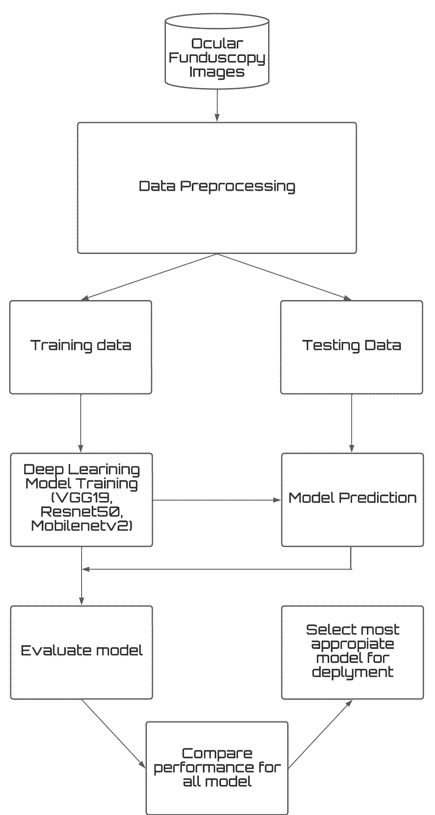
\includegraphics[scale=1]{3.png}
    \caption{Working steps}
    \label{Working steps}
\end{figure}
\section{Classification Using Resnet50}
ResNet50 is a variant of the Resnet model,, which has 48 convolution layers along with 1 MaxPool and 1 Average Pool layer. It has 3.8 x 109 floating point operations. It is a widely used ResNet model, and we have explored the ResNet50 architecture in depth. So as we can see in the resnet 50 architecture contains the following element:
\begin{enumerate}
    \item A convolution with a kernel size of 7 * 7 and 64 different kernels all with a stride of size 2 giving us 1 layer.
    \item Next we see max pooling with also a stride size of 2.
    \item In the next convolution there is a 1 * 1,64 kernel following this a 3 * 3,64 kernel and at last a 1 * 1,256 kernel, These three layers are repeated in total 3 time so giving us 9 layers in this step.
    \item Next we see kernel of 1 * 1,128 after that a kernel of 3 * 3,128 and at last a kernel of 1 * 1,512 this step was repeated 4 time so giving us 12 layers in this step.
    After that there is a kernal of 1 * 1,256 and two more kernels with 3 * 3,256 and 1 * 1,1024 and this is repeated 6 time giving us a total of 18 layers.
    \item And then again a 1 * 1,512 kernel with two more of 3 * 3,512 and 1 * 1,2048 and this was repeated 3 times giving us a total of 9 layers.
    \item We do a average pool and end it with a fully connected layer containing 1000 nodes and at the end a softmax function so this gives us 1 layer.
\end{enumerate}
\begin{figure}[H]
    \centering
    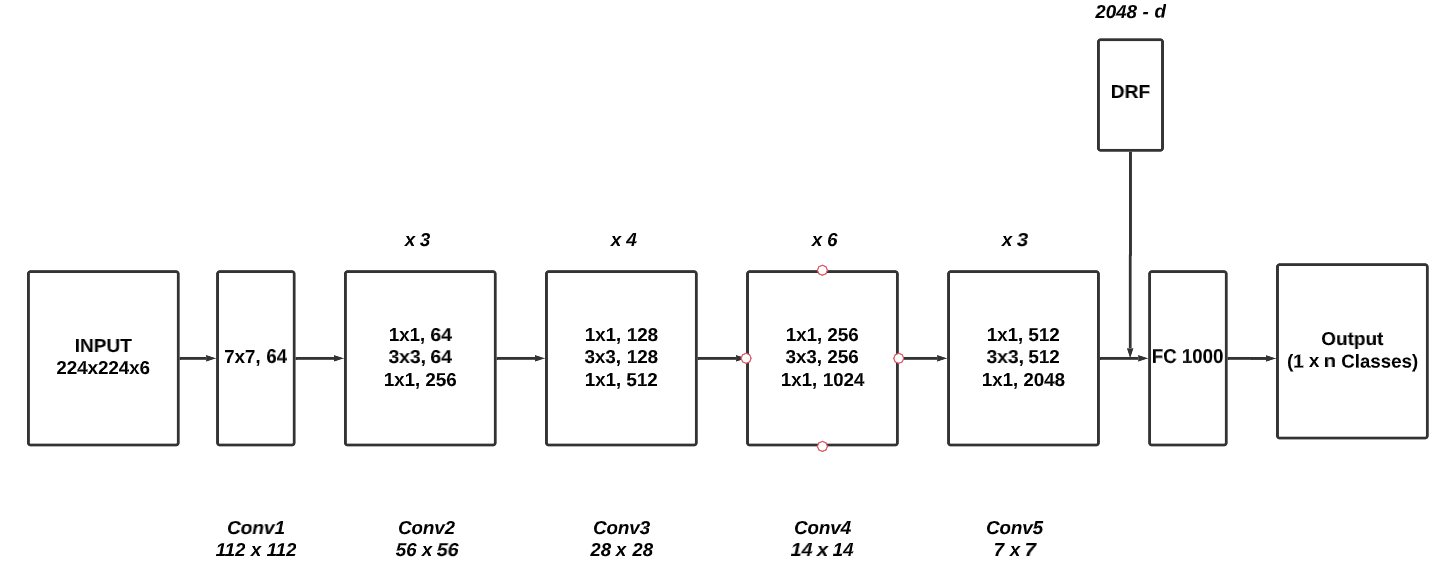
\includegraphics[scale=0.5]{40_Chapter_4/resnet50.png}
    \caption{Resnet50 Architecture}
    \label{Resnet50 Architecture}
\end{figure}
\section{Classification Using VGG19}
A variation of the VGG model called VGG19 has 19 layers in total (16 convolution layers, 3 Fully connected layer, 5 MaxPool layers and 1 SoftMax layer). There are further VGG variations, including VGG11, VGG16, and others. 19.6 billion FLOPs make up VGG19. So as we can see in the VGG19architecture contains the following element:
\begin{enumerate}
    \item A fixed size of (224 * 224) RGB image was given as input to this network which means that the matrix was of shape (224,224,3).
    \item The only preprocessing that was done is that they subtracted the mean RGB value from each pixel, computed over the whole training set.
    \item Used kernels of (3 * 3) size with a stride size of 1 pixel, this enabled them to cover the whole notion of the image.
    \item spatial padding was used to preserve the spatial resolution of the image.
    \item max pooling was performed over a 2 * 2 pixel windows with sride 2.
    \item this was followed by Rectified linear unit(ReLu) to introduce non-linearity to make the model classify better and to improve computational time as the previous models used tanh or sigmoid functions this proved much better than those.
    \item implemented three fully connected layers from which first two were of size 4096 and after that a layer with 1000 channels for 1000-way ILSVRC classification and the final layer is a softmax function.
\end{enumerate}
\begin{figure}[H]
    \centering
    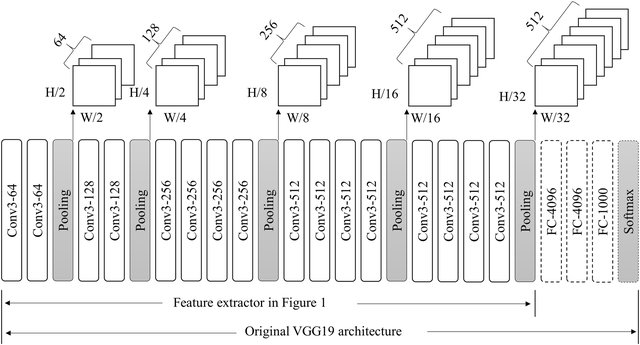
\includegraphics[scale=0.7]{40_Chapter_4/VGG19.jpg}
    \caption{VGG19 Architecture}
    \label{VGG19 Architecture}
\end{figure}
\vspace{5pt}
\section{Classification Using MobilenetV2}
We have explored MobileNet V2 architecture in depth. MobileNet V2 model has 53 convolution layers and 1 AvgPool with nearly 350 GFLOP. It has two main components:
\begin{enumerate}
    \item Bottleneck Residual Block
    \item Inverted Residual Block
\end{enumerate}
There are two types of Convolution layers in MobileNet V2 architecture:
\begin{enumerate}
    \item 1x1 Convolution
    \item 3x3 Depth wise Convolution 
\end{enumerate}
There are three streams and the input shape is 224x224. Our design involves a filter size of 32 for padding, a kernel size of 3, and activation function based on ReLU for the two first layers. The first max pooling layer has a pool size of 2 and strides of 2. The further plain layer combines all of the pooled characteristics into a separate cell. In the end, two thick layers were produced. The activation function for the first layer is ReLU, while the activation function for the least thick layer is softmax. The features are added to the network once they have been pre-processed. A bird's-eye perspective of the structure is shown below.
\begin{figure}[H]
    \centering
    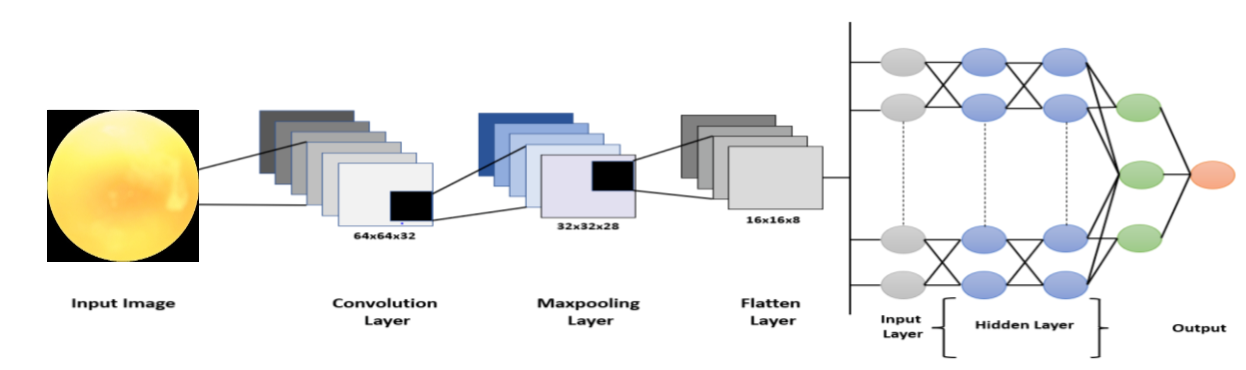
\includegraphics[scale=0.5]{40_Chapter_4/Mb2.png}
    \caption{MobileNetV2 Architecture}
    \label{MobileNetV2 Architecture}
\end{figure}
\vspace{5pt}
\section{Evaluation}
We should be prepared with several assessment metrics to examine the classification algorithm in the event of a classification problem. As follows:
\begin{enumerate}
    \item \textbf{Confusion Matrix:} The classification model's accuracy in classifying instances into distinct groups is summarized in a table called the confusion matrix. The model's anticipated label is on one axis of the confusion matrix, while the actual label is on the other. When comparing several models, we may use the confusion matrix to assess how well each one predicted true positives (TP) and true negatives (TN). We chose a model as our basic model if it accurately predicted TP and TN compared to other models.
\begin{figure}[H]
    \centering
    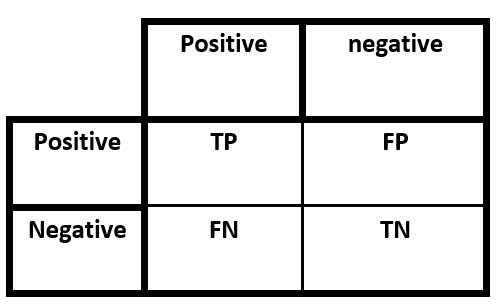
\includegraphics[scale=0.7]{40_Chapter_4/4.png}
    \caption{Confusion Matrix}
    \label{Confusion Matrix}
\end{figure}
TP = True Positive (The total number of images that are
correctly detected to be positive)\\
FP = False Positive (The total number of images that are
predicted to be positive but actually are negative)\\
TN = True Negative (The number of images that are
accurately predicted to be negative)\\
FN = False Negative (The number of images that are
incorrectly predicted to be negative)\\
    \item \textbf{Precision and Recall:} Precision and recall are two metrics used to evaluate classification and retrieval systems' performance. Precision is the percentage of relevant occurrences among all retrieved examples. Recall, also known as sensitivity, is the percentage of recovered instances among all appropriate models. In a perfect classifier, precision and recall are both one. 
\newline
\begin{align*}
Recall = \frac{TP}{TP+FP} 
\\
Precision = \frac{TP}{TP+FP}
\end{align*}
\newline
    \item \textbf{Accuracy:} It is calculated by dividing the total number of correctly categorized instances by the overall number of classified examples. When the importance of each class's prediction error is equal, this measure is crucial. Here, false positives should be addressed more than false negatives.
\newline
\begin{align*}
Accuracy = \frac{TP+tn}{TP+TN+FP+FN} 
\end{align*}
\newline
    \item \textbf{F1 score:} A weighted average of recall and accuracy is the F1 score. False positive and false negative results can occur in accuracy and recall, as is well known, thus both are taken into account. In most cases, the F1 score is more helpful than accuracy, particularly if your class is distributed unevenly. When false positives and false negatives cost about the same, accuracy performs best. It is preferable to include both Precision and Recall if the costs of false positives and false negatives are significantly different.
\newline
\begin{align*}
F1 Score = \frac{2*Recall*Precision}{Recall+Precision} 
\end{align*}
\newline
    \item \textbf{Learning Curve:} For algorithms that learn (optimize their internal parameters) gradually over time, like deep learning neural networks, learning curves are frequently employed in machine learning. If maximization is the metric used to measure learning, then higher scores (bigger numbers) signify more learning. Accuracy in categorisation might serve as an example. It is more typical to employ a score that minimizes, like loss or error, where better scores (lower numbers) imply greater learning and a value of 0.0 indicates that the training dataset was learnt properly with no errors. Additionally, a hold-out validation dataset that is separate from the training dataset can be used to test it. An assessment of the validation dataset provides insight into the model's "generalizability."
\end{enumerate}
\newpage
%\newpage\null\newpage
\chapter{EXPERIMENTAL RESULTS}
We will be analyze our model by there accuracy. Based on the input, or training, data, machine learning model accuracy is the statistic used to discover which model is best at recognizing correlations and patterns between variables in a dataset. The better predictions and insights a model can generate, which in turn provide more commercial value, depend on how well it can generalize to "unseen" data.
\vspace{5pt}
\begin{enumerate}
    \item \textbf{VGG19:} Using VGG-19, the accuracy of cataract vs. normal original data is 97.24\%. Glaucoma vs. normal has an accuracy of 90.94\%. In addition, myopia vs. normal has an accuracy of 98.13\%. The accuracy for hypertensive vs. normal is 94.73\%. It performed very well. We removed bias by balancing images for data classes.
    \vspace{5pt}
    \item \textbf{Resnet50:} Resnet50 is the best performed model according to accuracy. Using Resnet50, the accuracy of cataract vs. normal original data is 99.45\%. Glaucoma vs. normal has an accuracy of 90.98\%. In addition, myopia vs. normal has an accuracy of 99.26\%. The accuracy for hypertensive vs. normal is 94.73\%. It performed very well. We removed bias by balancing images for data classes.
    \vspace{5pt}
     \item \textbf{MobileNetV2:} It is the worst performed model out of three. The result without augmented data is too bad. But after taking augmented data, we did get satisfactory results form this model.
     \begin{enumerate}
         \item Cataract V Normal original data Using MobilenetV2 has 77\% accuracy.
         \item Cataract V Normal augmented data Using MobilenetV2 has 90\% accuracy 
         \item Glaucoma V Normal original data Using MobilenetV2 has 59\% accuracy 
         \item Glaucoma V Normal augmented data Using MobilenetV2 has 84\% accuracy 
         \item Myopia V Normal original data Using MobilenetV2 has 77\% accuracy 
         \item Myopia V Normal augmented data Using MobilenetV2 has 89\% accuracy 
         \item Hypertensive V Normal original data Using MobilenetV2 has 52\% accuracy 
         \item Hypertensive V Normal augmented data Using MobilenetV2 has 88\% accuracy 
     \end{enumerate}
\end{enumerate}
\vspace{5pt}
we can see in the training performance of MobileNetV2, its accuracy is getting improved and it can be inferred that the accuracy will certainly be improved if we run the training for more number of epochs. Also, There is hundred percentage training accuracy issue on VGG19  and Resnet50. We had tried to train those model in various dataset split ratio. There were various issue, but we selected the most optimized one. When we got hundred percentage training accuracy, we looked the accuracy of the model and the curve. If training accuracy curve is above validation curve and the accuracy was the highest, we recorded necessary information. But There is no hundred percent training accuracy issue on MobilenetV2. So, there is no overfitting issue also.\\
\\
\begin{figure}[H]
    \centering
    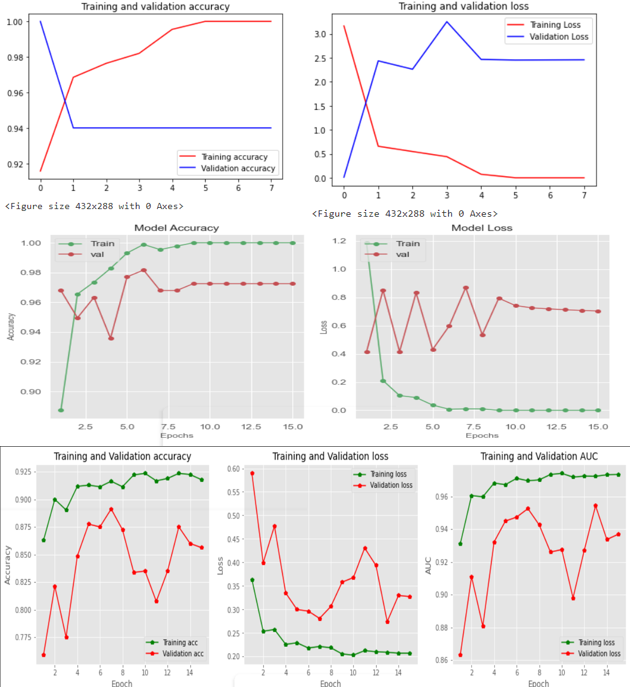
\includegraphics[scale=0.7]{c1.png}
    \caption{Plotting for Cataract v Normal.(Upper: Resnet50, Middle: VGG19, Lower: Mobilenetv2 on Augmented data)}
    \label{Plotting for Cataract v Normal}
\end{figure}
\vspace{5pt}
\\
\begin{figure}[H]
    \centering
    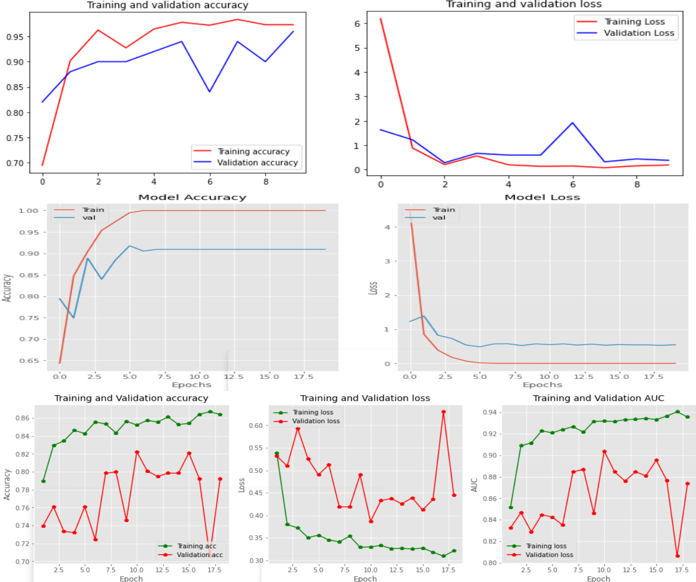
\includegraphics[scale=0.7]{c2.png}
    \caption{Plotting for Glaucoma v Normal.(Upper: Resnet50, Middle: VGG19, Lower: Mobilenetv2 on Augmented data)}
    \label{Plotting for Glaucoma v Normal}
\end{figure}
\vspace{5pt}

\begin{figure}[H]
    \centering
    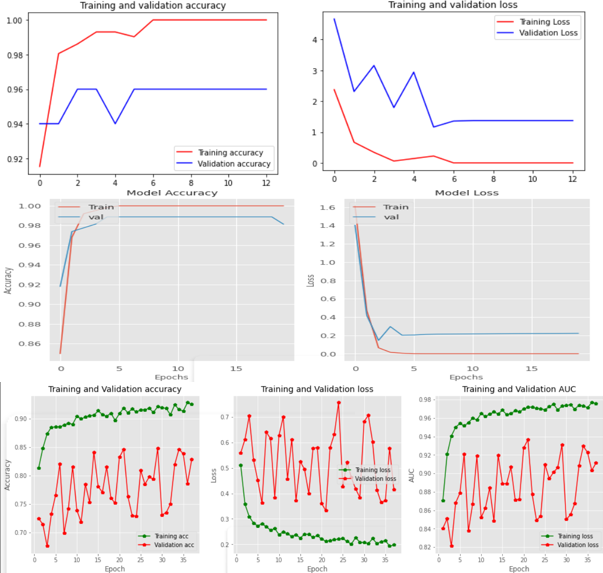
\includegraphics[scale=0.7]{c3.png}
    \caption{Plotting for Myopia v Normal.(Upper: Resnet50, Middle: VGG19, Lower: Mobilenetv2 on Augmented data)}
    \label{Plotting for Myopia v Normal}
\end{figure}
\vspace{5pt}

\begin{figure}[H]
    \centering
    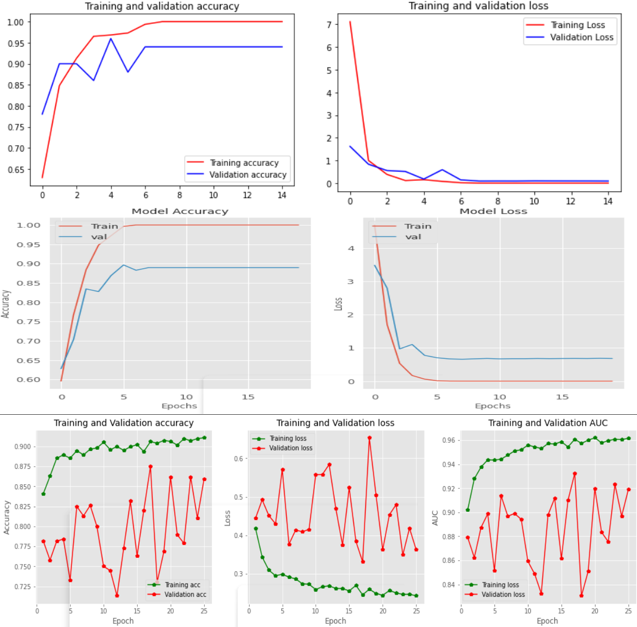
\includegraphics[scale=0.7]{c4.png}
    \caption{Plotting for Hypertensive v Normal.(Upper: Resnet50, Middle: VGG19, Lower: Mobilenetv2 on Augmented data)}
    \label{Plotting for Hypertensive v Normal}
\end{figure}
\begin{figure}[H]
    \centering
    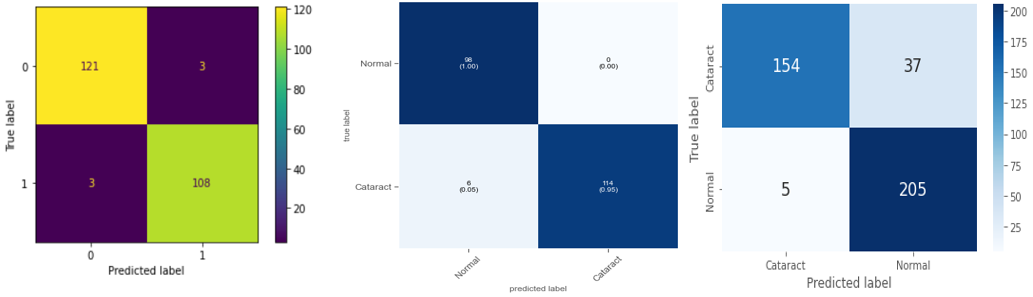
\includegraphics[scale=0.7]{50_Chapter_5/CNC.png}
    \caption{Confusion Matrix for Cataract v Normal.(Left: Resnet50, Middle: VGG19, Right: Mobilenetv2 on Augmented data)}
    \label{CNC}
\end{figure}
\begin{figure}[H]
    \centering
    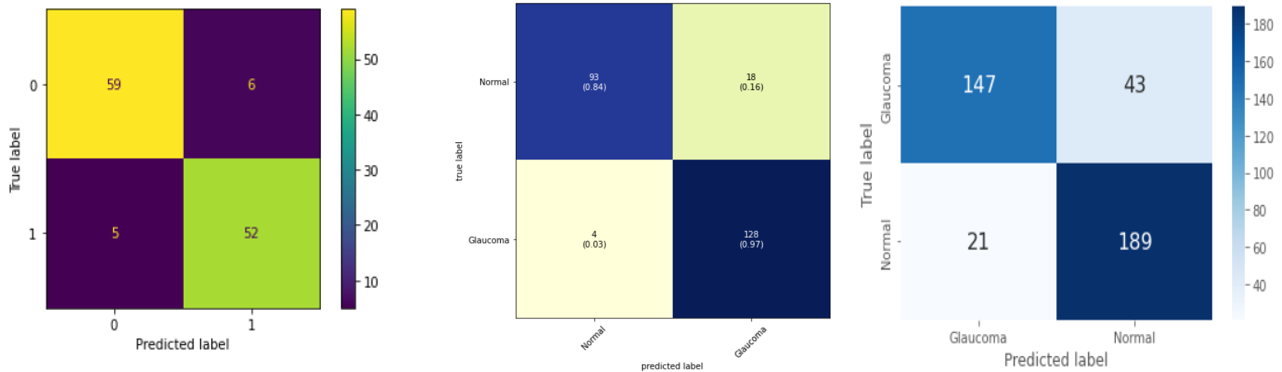
\includegraphics[scale=0.55]{50_Chapter_5/GNC.png}
    \caption{Confusion Matrix for Glaucoma v Normal.(Left: Resnet50, Middle: VGG19, Right: Mobilenetv2 on Augmented data)}
    \label{GNC}
\end{figure}
\begin{figure}[H]
    \centering
    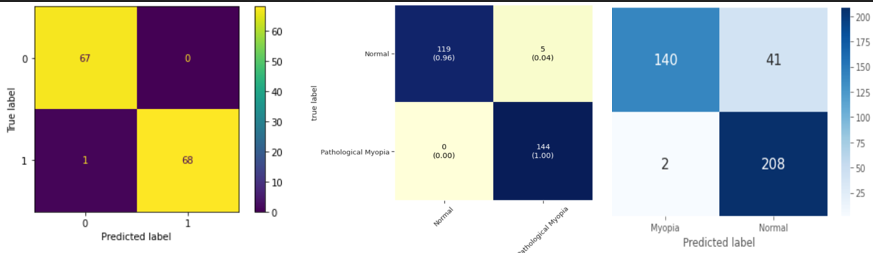
\includegraphics[scale=0.7]{50_Chapter_5/MNC.png}
    \caption{Confusion Matrix for Myopia v Normal.(Left: Resnet50, Middle: VGG19, Right: Mobilenetv2 on Augmented data)}
    \label{MNC}
\end{figure}
\begin{figure}[H]
    \centering
    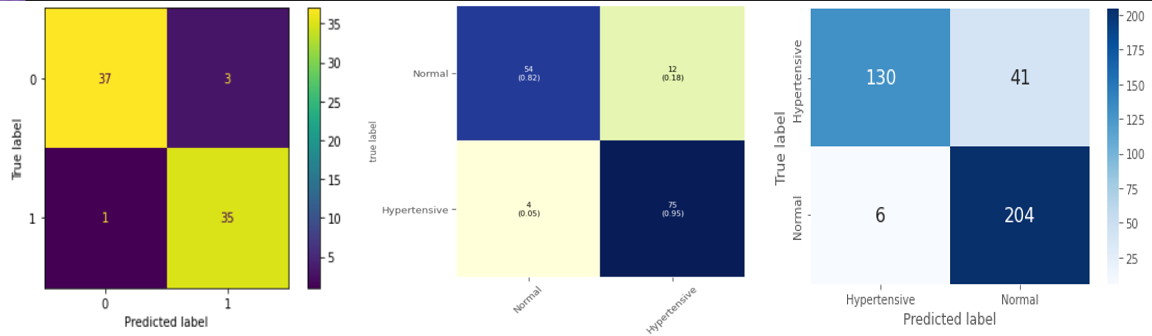
\includegraphics[scale=0.55]{50_Chapter_5/HNC.png}
    \caption{Confusion Matrix for Hypertensive v Normal.(Left: Resnet50, Middle: VGG19, Right: Mobilenetv2 on Augmented data)}
    \label{HNC}
\end{figure}
It is crucial to compare machine learning algorithms. Better performance of the machine learning software or solution is unquestionably the main goal of model comparison and selection. The goal is to select the fewest algorithms possible that meet the needs of the company and the data. If the chosen model fails to comprehend unknown input and is strongly associated with the training data, high performance may be short-lived. Finding a model that comprehends underlying data patterns is crucial in order to ensure that predictions are reliable and that little retraining is required. Minute details and information are captured when models are reviewed and prepared for comparisons, and they are useful during retraining.With the model information at hand, it is simple to focus on models that can provide fast processing and make efficient use of memory resources. Additionally, a number of parameters must be configured for the machine learning solutions throughout production.\\
\begin{table}[H]
\caption{MobileNetV2's Results Report without Augmented Data}
    \centering
    \begin{tabular}{|l|l|l|}
    \hline
        Model &  Accuracy \\ \hline
        Normal VS Cataract &  77\% \\ \hline
        Normal VS Glaucoma &  59\% \\ \hline
        Normal VS Myopia & 77\% \\ \hline
        Normal VS Hypertensive &  52\% \\ \hline
    \end{tabular}
\end{table}
\begin{table}[H]
\caption{Resnet50's Classification Report}
\centering
\begin{tabular}{|l|l|l|l|l|l|} 
\hline
Model                               & Accuracy                 & Disease              & Precision            & F1-score             & Recall                \\ 
\hline
\multirow{2}{*}{Normal VS Cataract} & \multirow{2}{*}{99.45\%} & Normal               & 0.98                 & 0.98                 & 0.98                  \\ 
\cline{3-6}
                                    &                          & Cataract             & 0.97                 & 0.97                 & 0.97                  \\ 
\hline
\multirow{2}{*}{Normal VS Glaucoma} & \multirow{2}{*}{90.98\%} & Normal               & 0.92                 & 0.91                 & 0.91                  \\ 
\cline{3-6}
                                    &                          & Glaucoma             & 0.9                  & 0.9                  & 0.91                  \\ 
\hline
Normal VS                           & \multirow{2}{*}{99.26\%} & Normal               & 0.99                 & 0.99                 & 1                     \\ 
\cline{3-6}
Myopia                              &                          & Myopia               & 1                    & 0.99                 & 0.99                  \\ 
\hline
Normal VS                           & \multirow{2}{*}{94.73\%} & Normal               & 0.97                 & 0.95                 & 0.93                  \\ 
\cline{3-6}
Hypertensive                        &                          & Hypertensive         & 0.92                 & 0.95                 & 0.97                  \\ 
\hline
\multicolumn{1}{l}{}                & \multicolumn{1}{l}{}     & \multicolumn{1}{l}{} & \multicolumn{1}{l}{} & \multicolumn{1}{l}{} & \multicolumn{1}{l}{} 
\end{tabular}
\end{table}
\begin{table} [H]
\caption{VGG19's Classification Report}
\centering
\begin{tabular}{|l|l|l|l|l|l|} 
\hline
Model                               & Accuracy                 & Disease              & Precision            & F1-score             & Recall                \\ 
\hline
\multirow{2}{*}{Normal VS Cataract} & \multirow{2}{*}{97.24\%} & Normal               & 0.94                 & 0.97                 & 1                     \\ 
\cline{3-6}
                                    &                          & Cataract             & 1                    & 0.97                 & 0.95                  \\ 
\hline
\multirow{2}{*}{Normal VS Glaucoma} & \multirow{2}{*}{90.94\%} & Normal               & 0.96                 & 0.89                 & 0.84                  \\ 
\cline{3-6}
                                    &                          & Glaucoma             & 0.88                 & 0.92                 & 0.997                 \\ 
\hline
Normal VS                           & \multirow{2}{*}{98.13\%} & Normal               & 1                    & 0.98                 & 0.96                  \\ 
\cline{3-6}
Myopia                              &                          & Myopia               & 0.97                 & 0.98                 & 1                     \\ 
\hline
Normal VS                           & \multirow{2}{*}{88.96\%} & Normal               & 0.97                 & 0.95                 & 0.93                  \\ 
\cline{3-6}
Hypertensive                        &                          & Hypertensive         & 0.92                 & 0.95                 & 0.97                  \\ 
\hline
\multicolumn{1}{l}{}                & \multicolumn{1}{l}{}     & \multicolumn{1}{l}{} & \multicolumn{1}{l}{} & \multicolumn{1}{l}{} & \multicolumn{1}{l}{} 
\end{tabular}
\end{table}
\begin{table}[H]
\caption{MobileNetV2's Classification Report with Augmented Data}
\centering
\begin{tabular}{|l|l|l|l|l|l|} 
\hline
Model                               & Accuracy                 & Disease              & Precision            & F1-score             & Recall                \\ 
\hline
\multirow{2}{*}{Normal VS Cataract} & \multirow{2}{*}{89.53\%} & Normal               & 0.85                 & 0.91                 & 0.98                  \\ 
\cline{3-6}
                                    &                          & Cataract             & 0.97                 & 0.88                 & 0.81                  \\ 
\hline
\multirow{2}{*}{Normal VS Glaucoma} & \multirow{2}{*}{84.00\%} & Normal               & 0.81                 & 0.86                 & 0.9                   \\ 
\cline{3-6}
                                    &                          & Glaucoma             & 0.88                 & 0.82                 & 0.77                  \\ 
\hline
Normal VS                           & \multirow{2}{*}{89.00\%} & Normal               & 0.84                 & 0.91                 & 0.99                  \\ 
\cline{3-6}
Myopia                              &                          & Myopia               & 0.99                 & 0.87                 & 0.77                  \\ 
\hline
Normal VS                           & \multirow{2}{*}{87.66\%} & Normal               & 0.83                 & 0.9                  & 0.97                  \\ 
\cline{3-6}
Hypertensive                        &                          & Hypertensive         & 0.96                 & 0.85                 & 0.76                  \\ 
\hline
\multicolumn{1}{l}{}                & \multicolumn{1}{l}{}     & \multicolumn{1}{l}{} & \multicolumn{1}{l}{} & \multicolumn{1}{l}{} & \multicolumn{1}{l}{} 
\end{tabular}
\end{table}

\newpage
\chapter{DEPLOYMENT}
The process of integrating a machine learning model into an already-existing production environment is known as deployment, and it allows you to use data to make useful business choices. It can be one of the most challenging stages of the machine learning life cycle and is one of the final ones. Frequently, traditional model-building languages are incompatible with an organization's IT systems, requiring data scientists and programmers to spend considerable time and brainpower rebuilding them. A model must be successfully put into production before it can be used for making useful decisions. The effect of your model will be much diminished if you are unable to consistently derive useful insights from it.Machine learning models must be smoothly deployed into production in order for businesses to use them to start making useful judgments. This will maximize their worth.\\ 

\begin{figure}[H]
    \centering
    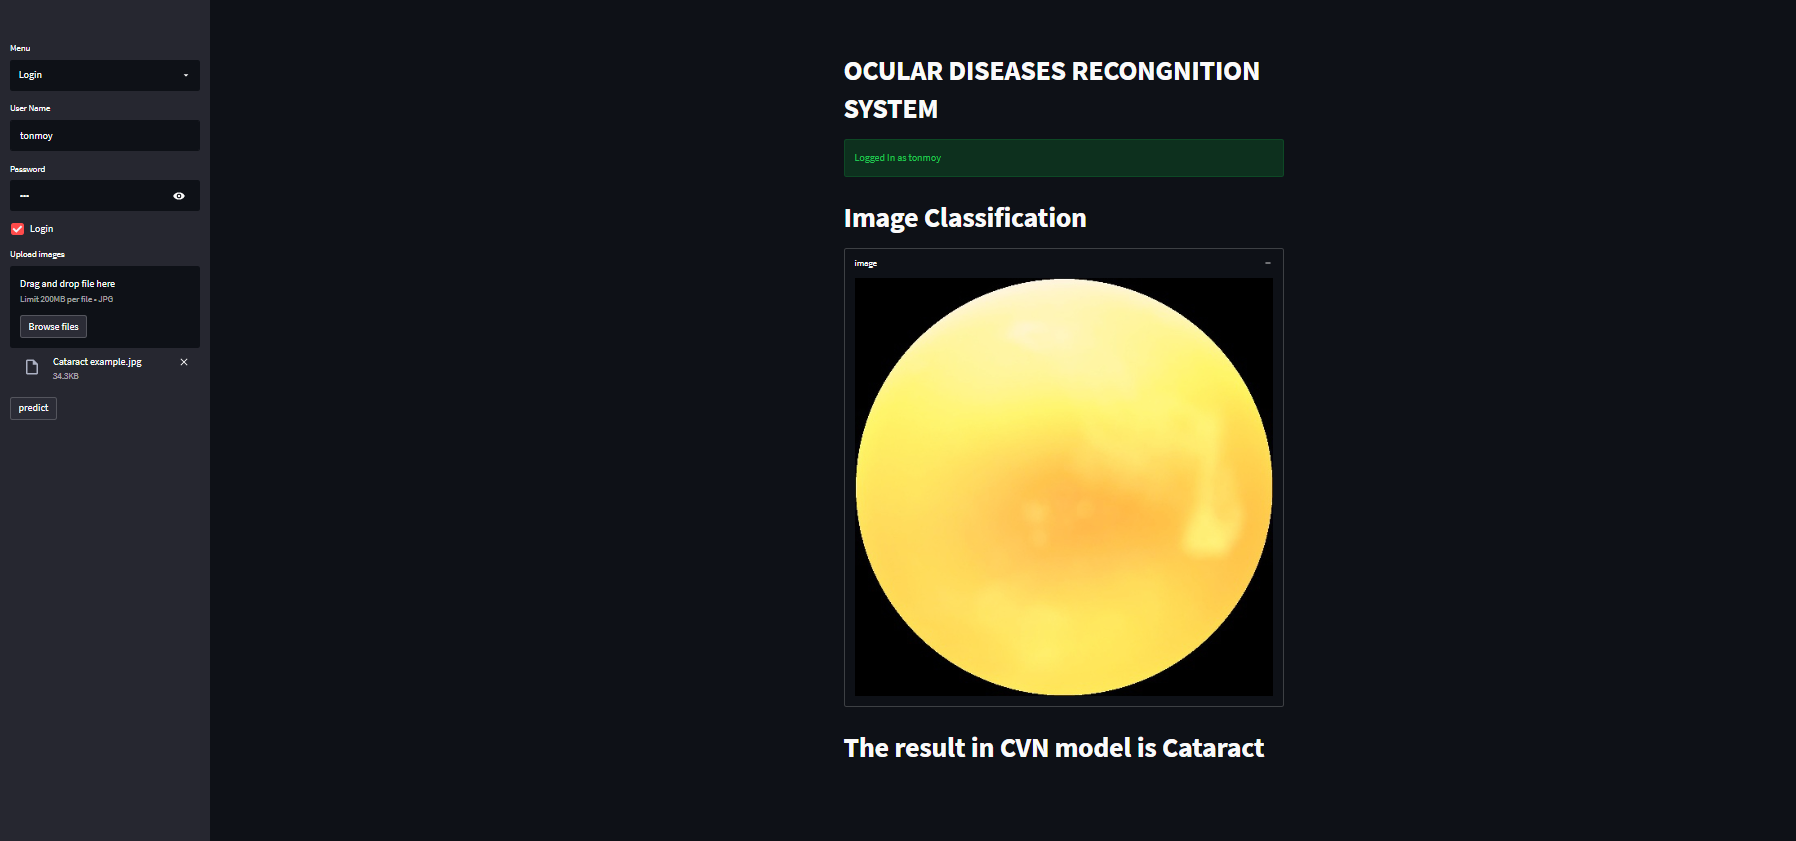
\includegraphics[scale=0.4]{70_Deployment/Deploy.png}
    \caption{Deployment}
    \label{deploy}
\end{figure}

A Python-based open source app framework is called Streamlit. It enables us to quickly develop web applications for data science and machine learning. Major Python libraries like scikit-learn, Keras, PyTorch, SymPy (latex), NumPy, pandas, and Matplotlib are all compatible with it. We used Streamlit to deploy our project.
We use Sqlite3 for temporary Data Management. Python SQLite3 module is used to integrate the SQLite database with Python. It is a standardized Python DBI API 2.0 and provides a straightforward and simple-to-use interface for interacting with SQLite databases. There is no need to install this module separately as it comes along with Python after the 2.5x version.

\newpage
%\newpage\null\newpage
\chapter{CONCLUSION}

In this study, we created four neural network-based models for classifying eye diseases. These models are VGG-19, Resnet-50, and MobileNetV2. When it comes to categorizing ocular disorders from fundus pictures, the Resnet50 offered the best accuracy for all models. The other models' performance was similarly acceptable. MobilenetV2 has no issue with hundred percent training accuracy. To verify the efficacy of our suggested strategy, we conducted extensive tests using the ODIR- 2019 dataset, which is open to the general public. In comparison to the current CNN-based ocular illness classification models, our suggested technique can produce results that are more spectacular while using less computing power. The nicest thing about our suggested approach is how easy it may be applied to various kinds of illness categorization based on medical images. Such a method will change the area of visual illness diagnostics and be of enormous use to medical experts.Additionally, this work could benefit from the use of ocular image segmentation. To address the imbalance issue, research can create comparable pictures of eye illness using generative adversarial networks (GANs). Additionally, a system like this would revolutionize the field of diagnosing eye diseases and be very helpful to medical professionals. Our opinion is that it can still be a valuable model, and there will likely be possibilities to improve it with further research and study in the near future.

\section{Data Availability}
The data used to support the findings of this study are freely available at https://www.kaggle.com/andrewmvd/ocular-disease-recognition-odir5k.

\newpage

%%%%%% Appendices %%%%%%
\appendix
\renewcommand{\chaptername}{Appendix}
\addtocontents{toc}{\protect\renewcommand{\protect\cftchappresnum}{\chaptername~}}
%%%%% Creating Appendix A
\chapter{CODE}
\label{appendix_0}
\graphicspath{{100_Appendices/}}

\section{Deployment Code}
\begin{lstlisting} [language=Python, caption=app.py]
import streamlit as st
import pandas as pd

# Security
#passlib,hashlib,bcrypt,scrypt
import hashlib
def make_hashes(password):
    return hashlib.sha256(str.encode(password)).hexdigest()

def check_hashes(password,hashed_text):
    if make_hashes(password) == hashed_text:
        return hashed_text
    return False
# DB Management
import sqlite3 
conn = sqlite3.connect('data.db')
c = conn.cursor()
# DB  Functions
def create_usertable():
    c.execute('CREATE TABLE IF NOT EXISTS 
    userstable(username TEXT,password TEXT)')

def add_userdata(username,password):
    c.execute('INSERT INTO userstable(username,password) 
    VALUES (?,?)',(username,password))
    conn.commit()

def login_user(username,password):
    c.execute('SELECT * FROM userstable 
    WHERE username =? AND password = ?',(username,password))
    data = c.fetchall()
    return data

def view_all_users():
    c.execute('SELECT * FROM userstable')
    data = c.fetchall()
    return data

def main():
    """OCULAR DISEASES RECONGNITION SYSTEM"""
    st.title("OCULAR DISEASES RECONGNITION SYSTEM")
    menu = ["Login","SignUp"]
    choice = st.sidebar.selectbox("Menu",menu)
    if choice == "Login":
        username = st.sidebar.text_input("User Name")
        password = st.sidebar.text_input("Password",type='password')
        if st.sidebar.checkbox("Login"):
            # if password == '12345':
            create_usertable()
            hashed_pswd = make_hashes(password)
            result= 
            login_user(username,check_hashes(password,hashed_pswd))
            if result:
                st.success("Logged In as {}".format(username))
                # Custom imports 
                import tensorflow as tf
                import numpy as np
                from PIL import Image, ImageOps
                st.title("Image Classification")
                upload_file = st.sidebar.file_uploader(
                "Upload images", type = 'jpg')
                generate_pred = st.sidebar.button("predict")
                model = tf.keras.models.load_model('CVN.h5')
                def import_n_pred(image_data, model):
                    size = (224,224)
                    image = ImageOps.fit
                    (image_data, size, Image.ANTIALIAS)
                    img = np.asarray(image)
                    reshape = img[np.newaxis,...]
                    pred = model.predict(reshape)
                    return pred
                if generate_pred:
                    image = Image.open(upload_file)
                    with st.expander('image', expanded=True):
                        st.image(image, use_column_width=True)
                    pred = import_n_pred(image, model)
                    labels = ['Cataract' , 'Normal']
                    st.title("The result in CVN model is {}"
                    .format(labels[np.argmax(pred)]))
                    if (np.argmax(pred)==1):
                        model = tf.keras.models.load_model
                        ('GVN.h5')
                        pred = import_n_pred(image, model)
                        labels = ['Glaucoma' , 'Normal']
                        st.title("The result in GVN model is {}"
                        .format(labels[np.argmax(pred)]))
                        if (np.argmax(pred)==1):
                            model = tf.keras.models.load_model
                            ('MVN.h5')
                            pred = import_n_pred(image, model)
                            labels = ['Myopia' , 'Normal']
                            st.title("The result in MVN model is {}"
                            .format(labels[np.argmax(pred)]))
                            if (np.argmax(pred)==1):
                                model = tf.keras.models.load_model
                                ('HVN.h5')
                                pred = import_n_pred(image, model)
                                labels = ['Hypertensive','Normal']
                                st.title("The result in HVN model is {}"
                                .format(labels[np.argmax(pred)]))
            else:
                st.warning("Incorrect Username/Password")

    elif choice == "SignUp":
        st.subheader("Create New Account")
        new_user = st.text_input("Username")
        new_password = st.text_input("Password",type='password')

        if st.button("Signup"):
            create_usertable()
            add_userdata(new_user,make_hashes(new_password))
            st.success("You have successfully created a valid Account")
            st.info("Go to Login Menu to login")

if __name__ == '__main__':   	
    main()
\end{lstlisting}
\newpage
% \null\newpage

\setstretch{1}

\vspace{12pt}
\begin{thebibliography}{00}
\bibitem{b1} Bourne, R. R., Stevens, G. A., White, R. A., Smith, J. L., Flaxman, S. R., Price, H., Jonas, J. B., Keeffe, J., Leasher, J., Naidoo, K., Pesudovs, K., Resnikoff, S., & Taylor, H. R. (2013). Causes of vision loss worldwide, 1990–2010: a systematic analysis. The Lancet Global Health, 1(6). https://doi.org/10.1016/s2214-109x(13)70113-x 
\bibitem{b2} Sommer, A., Tielsch, J. M., Katz, J., Quigley, H. A., Gottsch, J. D., Javitt, J. C., Martone, J. F., Royall, R. M., Witt, K. A., & Ezrine, S. (1991). Racial Differences in the Cause-Specific Prevalence of Blindness in East Baltimore. New England Journal of Medicine, 325(20), 1412–1417. https://doi.org/10.1056/nejm199111143252004 
\bibitem{b3} Congdon, N., O'Colmain, B., Klaver, C. C., Klein, R., Muñoz, B., Friedman, D. S., Kempen, J., Taylor, H. R., Mitchell, P., & Eye Diseases Prevalence Research Group (2004). Causes and prevalence of visual impairment among adults in the United States. Archives of ophthalmology (Chicago, Ill. : 1960), 122(4), 477–485. 
\bibitem{b4} Application of Ocular Fundus Photography and Angiography. (2014). Ophthalmological Imaging and Applications, 154–175. https://doi.org/10.1201/b17026-12 
\bibitem{b5} Rowe, S., MacLean, C. H., & Shekelle, P. G. (2004). Preventing Visual Loss From Chronic Eye Disease in Primary Care. JAMA, 291(12), 1487. https://doi.org/10.1001/jama.291.12.1487 
\bibitem{b6} Kessel, L., Erngaard, D., Flesner, P., Andresen, J., Tendal, B., & Hjortdal, J. (2015). Cataract surgery and age‐related macular degeneration. An evidence‐based update. Acta Ophthalmologica, 93(7), 593–600. https://doi.org/10.1111/aos.12665Li, N., Li, T., Hu, C., Wang, K.
\bibitem{b7} Li, N., Li, T., Hu, C., Wang, K., & Kang, H. (2021). A Benchmark of Ocular Disease Intelligent Recognition: One Shot for Multi-disease Detection. Benchmarking, Measuring, and Optimizing, 177–193. https://doi.org/10.1007/978-3-030-71058-3-11
\bibitem{b8}K. N. Alam, M. S. Khan, A. R. Dhruba et al., “Deep learning-based sentiment analysis of COVID-19 vaccination responses from Twitter data,” Computational and Mathematical Methods in Medicine, vol. 2021, pp. 1–15, 2021.
\bibitem{b9}J. He, C. Li, J. Ye, Y. Qiao, and L. Gu, “Self-speculation of clinical features based on knowledge distillation for accurate ocular disease classification,” Biomedical Signal Processing and Control, vol. 67, Article ID 102491, 2021.
\bibitem{b10}K. N. Alam and M. M. Khan, “CNN based COVID-19 prediction from chest X-ray images,” in Proceedings of the 2021 IEEE 12th Annual Ubiquitous Computing, Electronics & Mobile Communication Conference (UEMCON), pp. 0486–0492, IEEE, New York, USA, 1 December 2021.
\bibitem{b11}A. G. Roy, S. Conjeti, S. P. K. Karri et al., “ReLayNet: retinal layer and fluid segmentation of macular optical coherence tomography using fully convolutional networks,” Biomedical Optics Express, vol. 8, no. 8, pp. 3627–3642, 2017.
\bibitem{b12}C. S. Lee, A. J. Tyring, N. P. Deruyter, Y. Wu, A. Rokem, and A. Y. Lee, “Deep-learning based, automated segmentation of macular edema in optical coherence tomography,” Biomedical Optics Express, vol. 8, no. 7, pp. 3440–3448, 2017.
\bibitem{b13}S. P. K. Karri, D. Chakraborty, and J. Chatterjee, “Transfer learning based classification of optical coherence tomography images with diabetic macular edema and dry age-related macular degeneration,” Biomedical Optics Express, vol. 8, no. 2, pp. 579–592, 2017.
\bibitem{b14}M. Oda, T. Yamaguchi, H. Fukuoka, Y. Ueno, and K. Mori, “Automated Eye Disease Classification Method from Anterior Eye Image Using Anatomical Structure Focused Image Classification Technique,” 2020, https://arxiv.org/abs/2005.01433.
\bibitem{b15}F. Eperjesi, C. W. Fowler, and A. J. Kempster, “Luminance and chromatic contrast effects on reading and object recognition in low vision: a review of the literature,” Ophthalmic and Physiological Optics, vol. 15, no. 6, pp. 561–568, 1995.
\bibitem{b16}N. M. Dipu, S. Alam Shohan, and K. M. A. Salam, “Ocular disease detection using advanced neural network based classification algorithms,” ASIAN JOURNAL OF CONVERGENCE IN TECHNOLOGY, vol. 7, no. 2, pp. 91–99, 2021.
\bibitem{b17}M. S. Khan et al., “Deep learning for ocular disease recognition: An inner-class balance,” Comput. Intell. Neurosci., vol. 2022, p. 5007111, 2022.
\bibitem{b18} L. Jain, H. V. S. Murthy, C. Patel and D. Bansal, "Retinal Eye Disease Detection Using Deep Learning," 2018 Fourteenth International Conference on Information Processing (ICINPRO), 2018, pp. 1-6, doi: 10.1109/ICINPRO43533.2018.9096838.
\bibitem{b19} Nazir, T.; Irtaza, A.; Javed, A.; Malik, H.; Hussain, D.; Naqvi, R.A. Retinal Image Analysis for Diabetes-Based Eye Disease Detection Using Deep Learning. Appl. Sci. 2020, 10, 6185. https://doi.org/10.3390/app10186185
\bibitem{b20}Sarki, R., Ahmed, K., Wang, H. et al. Automated detection of mild and multi-class diabetic eye diseases using deep learning. Health Inf Sci Syst 8, 32 (2020). https://doi.org/10.1007/s13755-020-00125-5
\bibitem{b21} J. Shan and L. Li, "A Deep Learning Method for Microaneurysm Detection in Fundus Images," 2016 IEEE First International Conference on Connected Health: Applications, Systems and Engineering Technologies (CHASE), 2016, pp. 357-358, doi: 10.1109/CHASE.2016.12.
\bibitem{b22} Malik, S.; Kanwal, N.; Asghar, M.N.; Sadiq, M.A.A.; Karamat, I.; Fleury, M. Data Driven Approach for Eye Disease Classification with Machine Learning. Appl. Sci. 2019, 9, 2789. https://doi.org/10.3390/app9142789
\bibitem{b23} “Ocular disease recognition,” https://www.kaggle.com/andrewmvd/ocular-disease-recognition-odir5k.
\end{thebibliography}
\vspace{12pt}
\end{document}
